\chapter{Clustering}
\label{ch:capitolo2}

This chapter of the report aims at illustrating the clustering analysis performed on the dataset at hand.
The employed clustering techniques are K-means (Centroid-based), DBSCAN (density-based) and hierarchical clustering.

The analysis conducted using these methods focused on a selection of the continuous attributes of the dataset, which were appropriately log-transformed (when needed - as mentioned in subsection 1.3.2), and normalized using \texttt{MinMaxScaler}. 

% For the K-means algorithm, \texttt{totalNominations} and \texttt{totalMedia} were excluded due to their high proportion of zero values, which negatively affected cluster formation.
% In addition, an attempt was made to incorporate categorical variables to the analysis with the K-means algorithm by converting them into binary attributes and constructing a mixed-distances matrix. 
% Distances were then calculated using the Euclidean distance for numerical (log-tranformed and scaled) features and the Jaccard similarity for binary ones. 
% However, this approach was computationally expensive and did not lead to any improvement in the results.


\section{K-means}\label{sec:centroid_based}
%The clustering analysis performed with the K-means algorithm focused on the numeric variables of the dataset, excluding \texttt{awardWins}, \texttt{awardNominationsExcludeWins}, and \texttt{totalCredits} due to their high proportion of zero values, 
% which negatively affected cluster formation. 
%The variables have been appropriately log-transformed (as illustrated in the \textit{Variable Transformation} section) and normalized with \texttt{StandardScaler}.

Clustering analysis with K-means was performed using a carefully selected subset of features. 
This step was motivated by the algorithm's sensitivity to the curse of dimensionality, as including too many variables can negatively affect SSE and Silhouette scores.
For this reason, although only \texttt{numVotes}, \texttt{totalCredits}, \texttt{userReviewsTotal}, \texttt{runtimeMinutes}, and \texttt{criticReviewsTotal},
were chosen for this task, they proved to be a solid choice due to their ability to represent meaningful aspects of the data.
To identify the proper number of clusters, both SSE and Silhouette scores were evaluated. 
The objective was to find a configuration that reduces the SSE while maintaining a robust Silhouette score and a proper \textit{k}. 
The plots in Figure X show that \textit{k} = 4 provides a balance between the two values (obtaining SSE equal to 535.51 and 0.315 for the Silhouette score).
Only for visualization purposes, Principal Component Analysis (PCA) was employed. 
The first two components account for 58.01\% and 21.48\% of the total variance, indicating that this projection provides a fairly informative view of the clustering structure. 
The cluster results are presented in figure~\ref{fig:kmeans_visualization}. 
The 4 distinct clusters appear well-separated, suggesting that K-means managed to capture meaningful groupings in the data.



% To identify the optimal number of clusters, both the SSE and Silhouette scores were computed. The goal was to find a configuration that minimizes the SSE while maintaining a robust Silhouette score and a proper \textit{k}. 
% The plots in figure~\ref{fig:sse_silh_kmeans} demonstrate that \textit{k} = ??? provides the optimal balance between these metrics. Choosing \textit{k} = ??? returns a SSE score of ??? and Silhouette score of ???. 
% \textbf{VALORI TROPPO ALTI, VEDERE SE CAMBIANO CAMBIANDO SCALING E/O TOGLIENDO OUTLIER}

% To visualize the clustering results, Principal Component Analysis (PCA) was employed. The plot in figure~\ref{fig:pca_kmeans} reveals that 4 principal components are enough to capture the optimal amount of variance for the selected variables, as evidenced by the the point where the line starts to flatten, indicating that adding more components doesn't increase explained variance significantly.
 

\begin{figure}[H]
    \centering
    \begin{subfigure}[b]{0.48\textwidth}
        \centering
        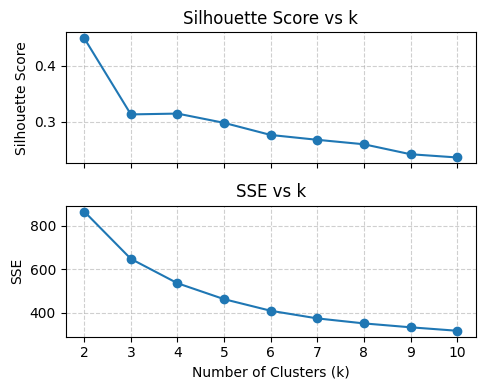
\includegraphics[width=\textwidth]{plots/sse_silh_kmeans_def.png}
        \caption{SSE and Silhouette scores}
        \label{fig:sse_silh_kmeans}
    \end{subfigure}
    \begin{subfigure}[b]{0.48\textwidth}
        \centering
        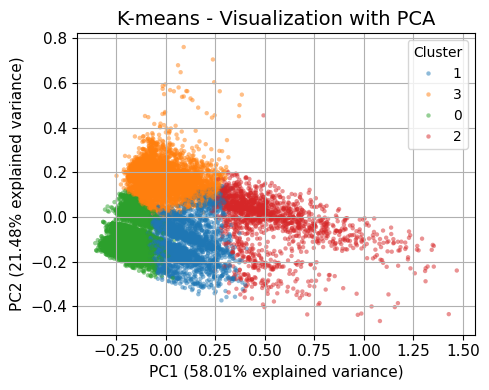
\includegraphics[width=\textwidth]{plots/kmeans_clusters.png}
        \caption{Clustering Visualization with PCA}
        \label{fig:kmeans_visualization}
    \end{subfigure}
    \caption{K-means - Cluster analysis}
    \label{fig:subplots_kmeans}
\end{figure}
% The distribution of data points across the four clusters is as follows (shown in percentage of data points per cluster):
% Red (0): 51.68\%, Blue (1): 7.42\%, Green (2): 24.22\%, Orange (3): 16.68\%.
% The clusters are not as well-separated in most Principal Component combinations as they are with PC1. 
% In fact, in the other combinations, the clusters tend to overlap and their boundaries are not always clearly distinct.
% This might be an indication that the true clusters have irregular shapes or different densities, resulting in boundaries between them being not clearly defined.



\section{DBSCAN}\label{sec:density_based}
To determine suitable DBSCAN parameters, the k-th distance plot was used as starting point (Figure~\ref{fig:dbscan_kth}). 
By varying \textit{k} (\textit{MinPts}) and observing the corresponding distance curves, the range between 0.08 and 0.2 was identified for a possible \textit{Eps} value.
The algorithm was applied to the following features: \texttt{numVotes}, \texttt{totalCredits}, \texttt{criticReviewsTotal}, \texttt{userReviewsTotal}, and \texttt{runtimeMinutes}. 
Although different combinations were tested, they all led to similar results. 
Effectively, initial experiments clearly revealed DBSCAN’s sensitivity to highly sparse and imbalanced datasets; 
in most cases, the algorithm produced a highly populated single cluster corresponding to the dominant dense region, 
while leaving the sparser regions largely unstructured.
\begin{figure}[H]
    \centering
    \begin{subfigure}[b]{0.48\textwidth}
        \centering
        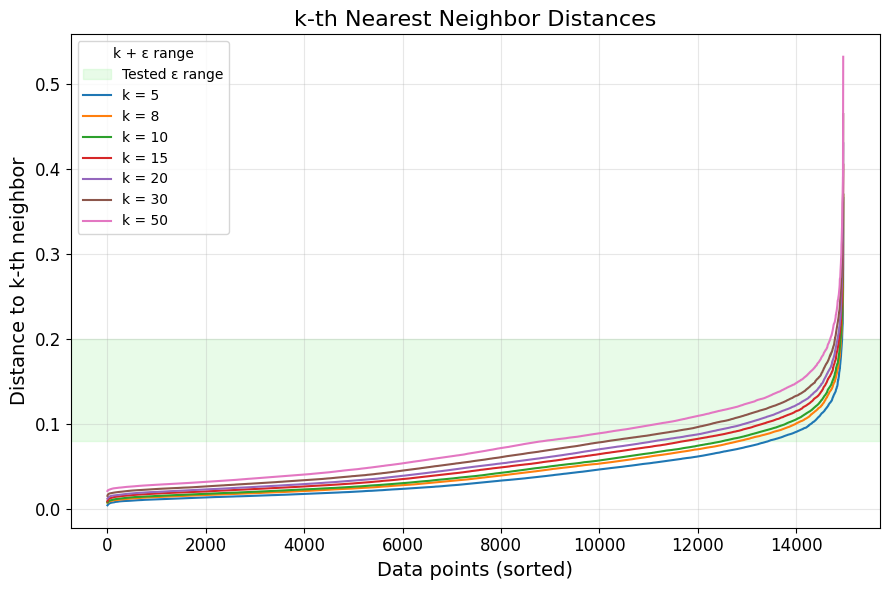
\includegraphics[width=\textwidth]{plots/dbscan_kth.png}
        \caption{K-th distance plot}
        \label{fig:dbscan_kth}
    \end{subfigure}
    \begin{subfigure}[b]{0.48\textwidth}
        \centering
        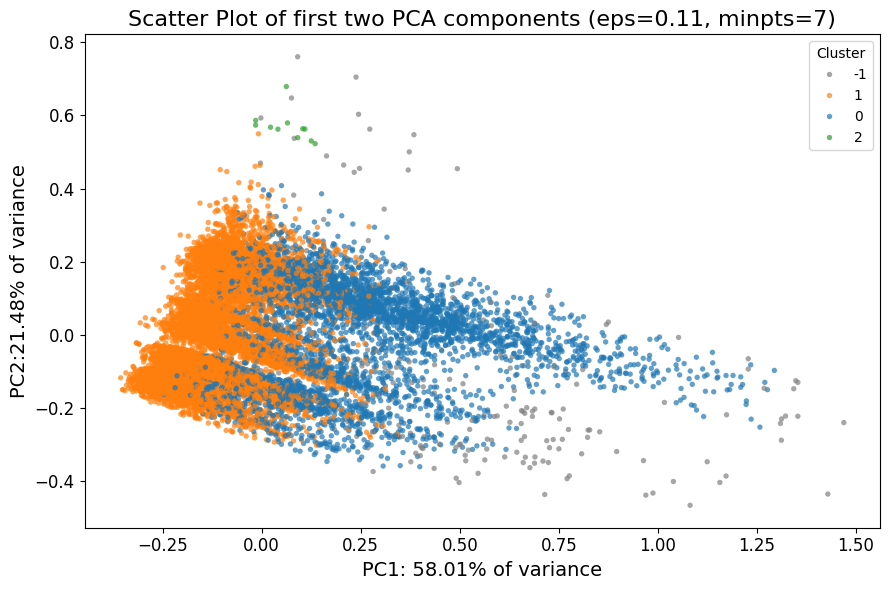
\includegraphics[width=\textwidth]{plots/dbscan_scatterplot.png}
        \caption{Visualization with PCA}
        \label{fig:dbscan_visualization}
    \end{subfigure}
    \caption{DBSCAN - Cluster analysis}
    \label{fig:subplots_DBSCAN}
\end{figure}

Initial experiments clearly revealed DBSCAN's sensibility towards high-sparsed and imbalanced dataset;
in most cases the algorithm produced an highly populated single cluster in correspondence of the dominant dense region, leaving sparser regions largely unstructured. 
To address this issue and obtain more meaningful clustering, different combination of \texttt{min\_eps} and \texttt{min\_points} in the following ranges were tested:
\begin{itemize}
    \item \texttt{eps\_list} =  [0.08, 0.09, 0.1, 0.12, 0.14, 0.16, 0.18, 0.2, 0.3, 0.4, 1.0];
    \item \texttt{min\_points\_list} =  [4, 5, 6, 7, 8, 9, 10, 11, 12, 13, 14, 15, 20].
\end{itemize}

Each combination was evaluated based on the number of clusters (with a minimum threshold of 2), size of the clusters, noise points, and silhouette score 
(filtered for values $>$ 0.1), excluding the cases where only one cluster was created, or where the silhouette value was consisidered too low.

% First of all it is interesting to report that setting \textit{Eps} value > 0.16 never led to the formation of more than one cluster, (for any \texttt{min\_points} tested). 
% Similarly, eps value between 0.13 and 0.16 consistently led to the collapse of most points into a single large cluster, with, occasionally, one/two minor residual clusters, (for any \texttt{min\_points} tested). \\

% Note that, in this context, the high Silhouette score is misleading, as it tends to favor cohesion of the main cluster, at the expense of structural granularity.
% On the other side the combination of lower epsilon values (as 0.10) and few \texttt{min\_pts} (4-5) 
% often resulted in over-fragmentation, producing several clusters of very few elements (5/6), typically corresponding to isolated outliers or noise points rather than meaningful groups.
% In general with \textit{Eps} values (between 0.09-0.12) the algorithm was able to differentiate between regions of varying density, as \textit{Eps} = 0.13 was identified as the threshold below which DBSCAN starts splitting the big cluster in two different ones.
% \textbf{- EVENT METTI GRAFICO-  as Shown in Figure X}\\

% In Table~\ref{tab:eps} the most interesting results are summarized.
% \begin{table}[h]
% \centering
% \begin{tabular}{llll}
% \toprule
% \textbf{eps threshold} & \textbf{Min points} & \textbf{Silhouette} & \textbf{Cluster composition}  \\
% \midrule
% \texttt{\textbf{$\varepsilon$} > 0.16} & for any tested \texttt{min\_points}  & valori  & never led to the formation of more than one cluster (for any \texttt{min\_points} tested) \\
% \texttt{0.13 $\leq$ \textbf{$\varepsilon$} < 0.16 } & for any tested \texttt{min\_points}&  valori  & consistently led to a single large cluster, with, occasionally, one/two minor residual clusters (for any \texttt{min\_points} tested)\\
% \texttt{0.11 $\leq$ \textbf{$\varepsilon$} < 0.13 } & for any tested \texttt{min\_points} & valori &  DBSCAN starts splitting the big cluster in two different ones, starting to differentiate differentiate between regions of varying density\\
% \texttt{\textbf{$\varepsilon$} < 0.11} & with lower \texttt{min\_points} (4, 5)& valori  & often resulted in over-fragmentation, producing several clusters of very few elements (5/6), typically corresponding to isolated outliers or noise points rather than meaningful groups.  \\

% \bottomrule
% \end{tabular}
% \caption{title}
% \label{tab:eps}
% \end{table}

Even if the configurations did not yield fully satisfactory results, in Table~\ref{tab:eps} the most interesting ones are summarized.
Note that, in this context, an high Silhouette score is misleading, as it tends to favor cohesion of the main cluster, at the expense of structural granularity.
\begin{table}[h]
% \hspace*{-0.5cm}
\centering
\begin{tabular}{llll}
\toprule
\textbf{eps threshold} & \textbf{Min points} & \textbf{Silhouette} & \textbf{Cluster composition}  \\
\midrule
\texttt{\textbf{$\varepsilon$} $>$ $0.16$} & for any tested value &  $>$ 0.51  & never led to more than one cluster \\
\texttt{$0.13$ $\leq$ \textbf{$\varepsilon$} $<$ $0.16$} & for any tested value &  $[0.49,\ 0.51]$  & led to one cluster and, occasionally, 1 or 2 minor ones\\
\texttt{\textbf{$\varepsilon$} $<$ $0.13$}& for any tested value & $[0.10,\ 0.28]$ & the big cluster it's splitted in two different ones \\
\texttt{\textbf{$\varepsilon$} $\leq$ $0.10$} & lower values $[4,\ 5]$& $[0.10,\ 0.22]$  & led to several, not meaningful, clusters of 5/6 points\\

\bottomrule
\end{tabular}
\caption{Relevant DBSCAN parameters configurations}
\label{tab:eps}
\end{table}



Exlcuding the combination with higher \textit{Eps} value, that made the points collaps into one cluster, and the ones with low \textit{Eps} and few \texttt{min\_pts} ,that resulted in over-fragmentation, 
the analysis focused on \textit{Eps} in the range $[0.11,\ 0.13)$.
Despite the limitations of the dataset structure, in this range the algorithm was able to differentiate between regions of varying density, 
% producing several clusters of very few elements (5/6), typically corresponding to isolated outliers or noise points rather than meaningful groups, 

One of the most interesting compromise (though still suboptimal in absolute terms) was found with \textit{Eps} = 0.11, \texttt{min\_points} = 7: 
As shown in (Figure~\ref{fig:dbscan_visualization}), this setting resulted in a 3 cluster structure: a compact cluster of 10378 points was extracted from the densest region, a less dense cluster with fewer points (4347) captured intermediate-density areas or mild outliers, 
and a very small one (only 11 points), but well-separated, cluster effectively captured a potential relevant local pattern. Only 219 points were labeled as noise, and the Silhouette Score was 0.2699.\\

\textbf{QUESTA PARTE VOLENDO PUò ANDARE NELLE CONSIDERAZIONI GENERALI}\\
To conclude, these observations highlight DBSCAN's limitations when applied to datasets with skewed feature distributions and unbalanced local densities.
Nonetheless, the exploration helped isolate parameter ranges where meaningful subclusters begin to emerge,beyond the dominant density mass.







% \begin{figure}[H]
%     \centering
%     \begin{subfigure}[b]{0.49\textwidth}
%         \centering
%         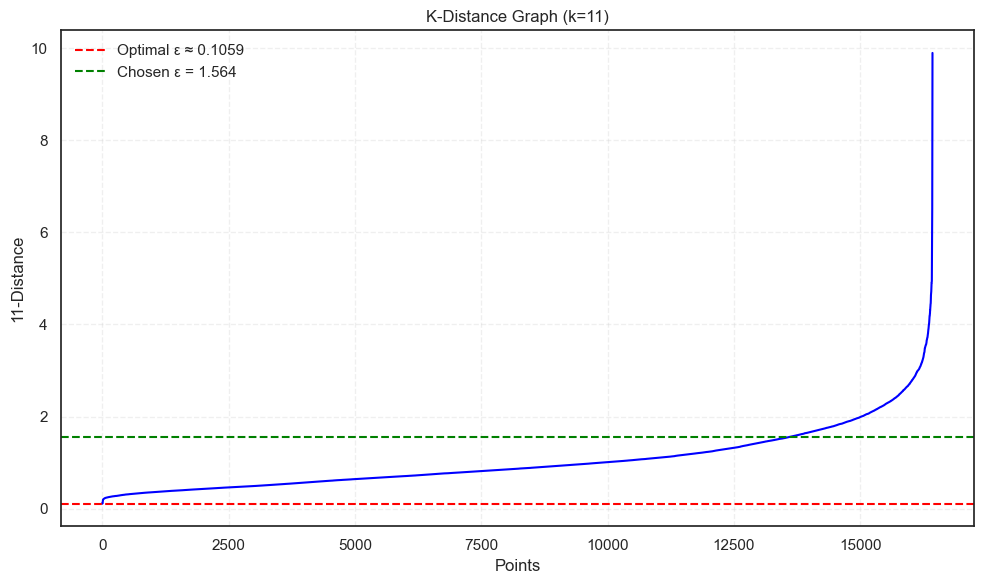
\includegraphics[width=\textwidth]{plots/DBSCAN_kth_graph.png}
%         \caption{k\textsuperscript{th} nearest neighbors}
%         \label{fig:DBSCAN_kth_graph}
%     \end{subfigure}
%     % \hfill
%     % \begin{subfigure}[b]{0.3\textwidth}
%     %     \centering
%     %     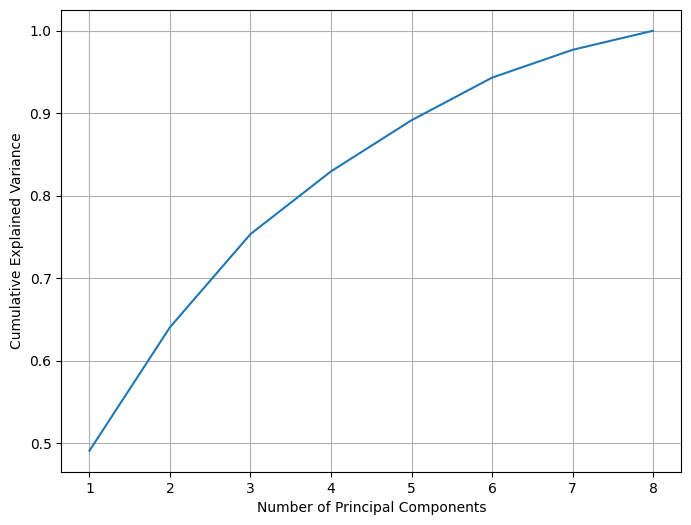
\includegraphics[width=\textwidth]{plots/pca_kmeans.png}
%     %     \caption{PCA Analysis}
%     %     \label{fig:pca_kmeans}
%     % \end{subfigure}
%     % \hfill
%     \begin{subfigure}[b]{0.49\textwidth}
%         \centering
%         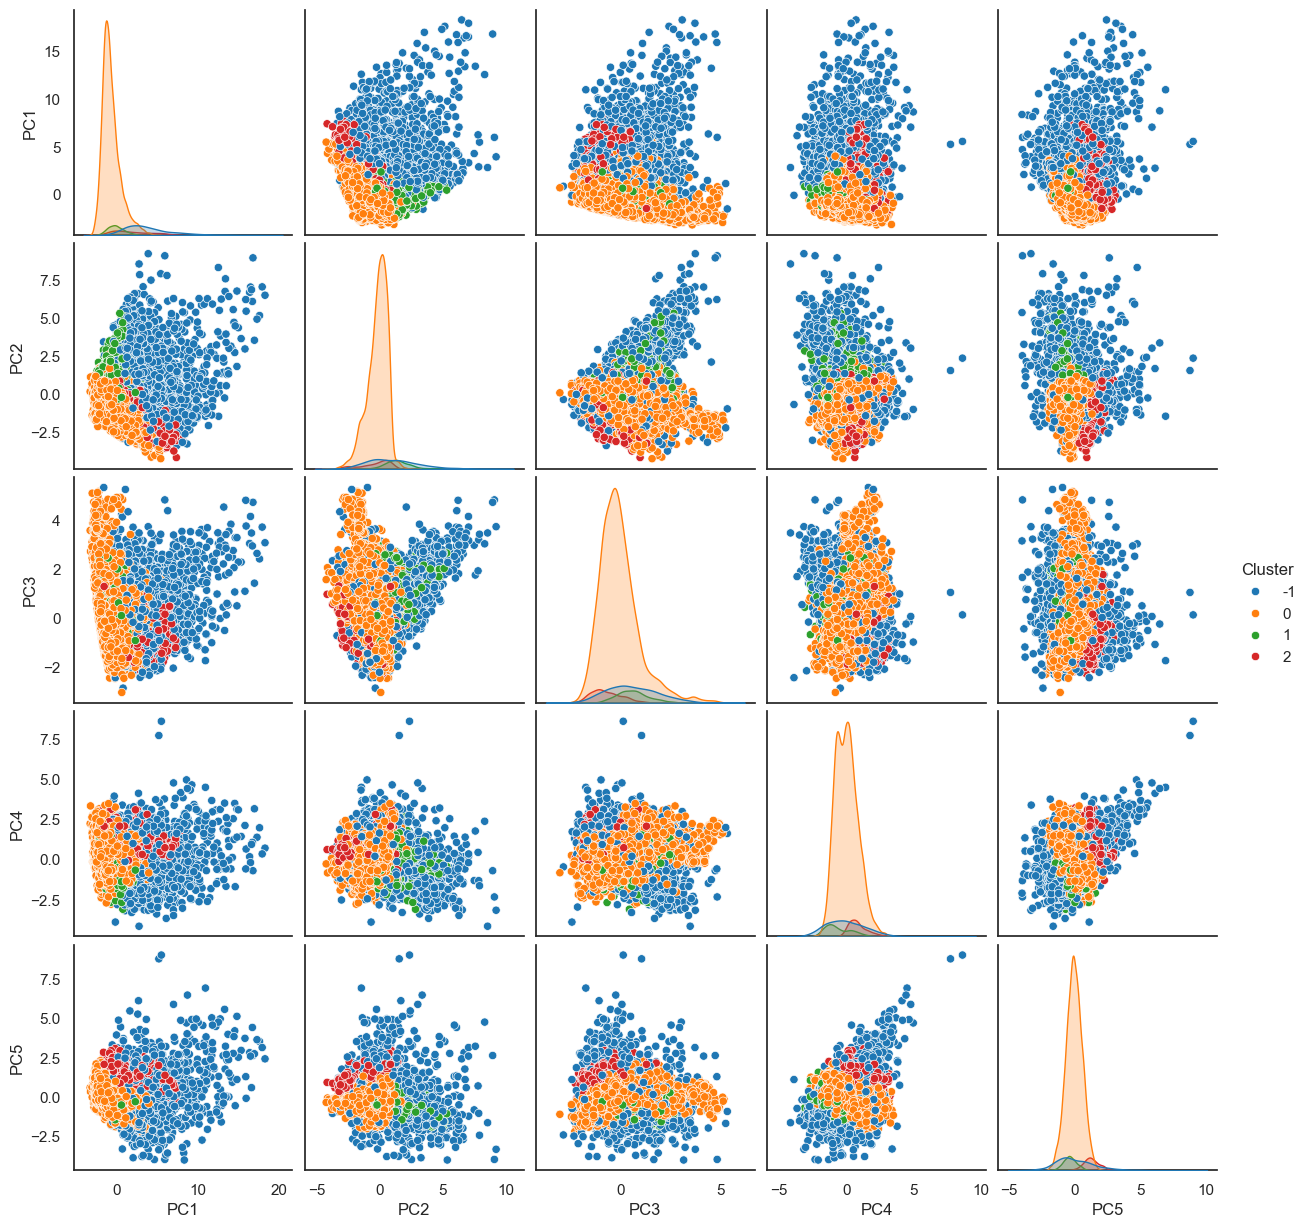
\includegraphics[width=\textwidth]{plots/DBSCAN_provvisoria.png}
%         \caption{DBSCAN Visualization}
%         \label{fig:DBSCAN_provvisoria}
%     \end{subfigure}
%     \caption{DBSCAN clustering analysis}
%     \label{fig:three_subplots}
% \end{figure}




\section{Hierarchical clustering}\label{sec:hierarchical}
Hierarchical clustering was performed using all linkages (Ward, Average, Complete, Single), with the Euclidean
distance metric. After a careful analysis of multiple clusterings, it was decided to procede with
all remaining numerical features, log transformed and normalized with \texttt{MinMaxScaler}.
Figure~\ref{fig:hier_clust_stats} shows the results of the analysis, which includes the Silhouette and SSE
scores, as well as the maximum and minimum percentage of points per cluster.
\begin{figure}[H]
    \centering
    % Left: Tall figure (a)
    \begin{subfigure}[t]{0.49\textwidth}
        \centering
        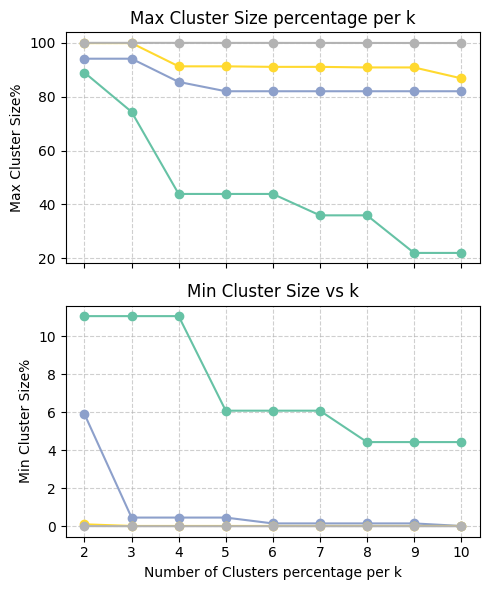
\includegraphics[width=0.95\textwidth]{plots/max_min_pctg.png}
        \subcaption{Max/Min percentage of points per cluster}
        \label{fig:max_min_pctg}
    \end{subfigure}
    \hfill
    \begin{subfigure}[t]{0.49\textwidth}
        \centering
        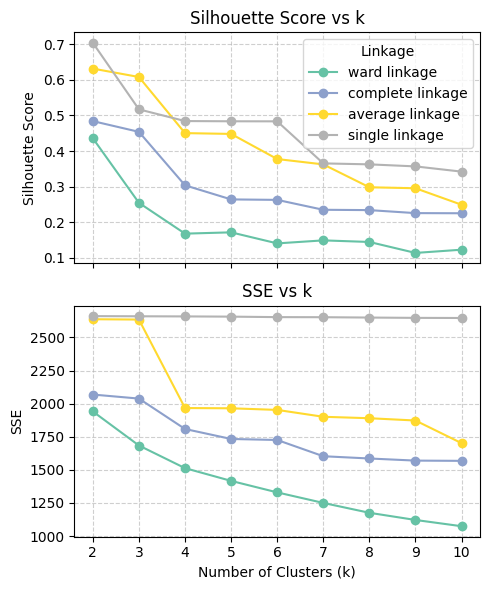
\includegraphics[width=0.95\textwidth]{plots/sil_sse_hierarchical_clust.png}
        \subcaption{Silhouette and SSE scores}
        \label{fig:sil_sse_hierarchical_clust}
    \end{subfigure}
    \caption{Hierarchical clustering metrics for different numbers of clusters}
    \label{fig:hier_clust_stats}
\end{figure}

From figure~\ref{fig:max_min_pctg}, it can be observed that Single linkage produces a single cluster which contains basically all data points. This makes it unsuitable for this use case.
Average and Complete linkages produce a cluster with a high maximum cluster size (above 90\% of the dataset for most
of the number of clusters tested for Average, and 80\% for Complete).
These results are likely due to two main causes: 
\begin{itemize}
    \item Usage of skewed features, which lead to areas with a very high density of points;
    \item High dimensionality of the dataset, which makes it more difficult to separate clusters effectively.
\end{itemize}

These issues are mitigated by Ward's method, which doesn't show a dominant biggest cluster, for
all numbers of clusters tested. The minimum cluster size is also consistently more balanced
across different numbers of clusters.\\


Since Ward's method is based on Squared Error, it's not surprising how its SSE is consistently lower than other linkages, as shown in the second graph of figure~\ref{fig:sil_sse_hierarchical_clust}.
What's more interesting is that Ward's method has the lowest Silhouette scores for all numbers
of clusters tested, which indicates that the clusters are not well separated. This is due to
the fact that Ward's method groups the data which resides in the high-density area
mentioned above into smaller clusters, leading to less well-defined boundaries between them.
In the next two sections, the results of Ward's method and Complete Linkage will be analyzed;
the other two will not be discussed further, as they provide limited insights on the dataset.

% By looking at Ward's statistics, the more interesting numbers of clusters to analyze are 4 and 5.
% The first one corresponds to a big decline in maximum cluster size (from 74 to 44\%),
% with a minimum cluster size of around 11\%; the second one has the same maximum cluster size but a smaller minimum cluster size (around 6\%), but has slightly higher Silhouette score
% (17.1\% against 16.8\% for 4 clusters) and a lower SSE. Figure~\ref{fig:dendrograms_ward} shows
% the dendrograms for the two clusterings.
\subsection{Ward's method}
Figure~\ref{fig:dendrograms_ward} a dendrogram and a scatter plot for a clustering obtained through
Ward's Method. Because of the parameters observed in the previous section, cleaner dendrograms,
as well as consistency with other clustering methods, the hierarchical clustering is cut at 4 clusters.
% Both clusterings are set to have 4 clusters, which in both cases leads to cleaner dendrograms.
\begin{figure}[H]
    \centering
    \begin{subfigure}[b]{0.49\textwidth}
        \centering
        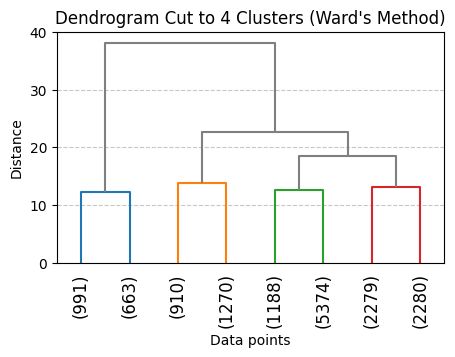
\includegraphics[width=\textwidth]{plots/dendrogram_4.png}
        \caption{Ward's Method Dendrogram}
        \label{fig:dendrogram_ward}
    \end{subfigure}
    \begin{subfigure}[b]{0.49\textwidth}
        \centering
        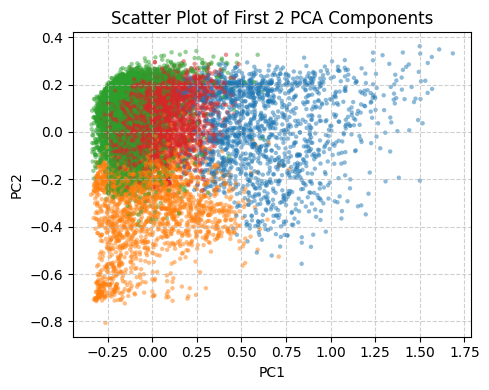
\includegraphics[width=\textwidth]{plots/scatter_ward.png}
        \caption{Ward's Method Scatter plot}
        \label{fig:scatter_ward}
    \end{subfigure}
    \caption{Ward's method clustering}
    \label{fig:dendrograms_ward}
\end{figure}

% The obtained dendrogram has clearly separated clusters, as shown in figure~\ref{fig:dendrogram_ward}.
% The clusters all form at a similar distance (around 12), meaning the SSE increase is similar for
% all clusters.
% It is interesting to note how the smallest cluster is merged with the others at the last merge; this,
% as can be observed in figure~\ref{fig:scatter_ward}, is the cluster which resides in the less dense area of the dataset.
% The other three clusters are closer to each other, as they are a result of the split of the higher density
% area of the dataset. Compared to K-Means, the clusters are not as cleanly separated in the PCA space,
% leading to overlapping areas between them.
The dendrogram in Figure~\ref{fig:dendrogram_ward} reveals well-separated clusters, all of which merge at a
similar linkage distance (approximately 12). This indicates that the increase in within-cluster sum of
squares (SSE) is relatively consistent across all cluster merges, as expected from Ward's method.
Notably, the smallest cluster is the last to be merged, which suggests it is more distinct from the others.
As shown in Figure~\ref{fig:scatter_ward}, this cluster lies in a sparser region of the dataset.
In contrast, the remaining three clusters originate from the denser region, and are therefore spatially
closer to one another.
Compared to K-Means, the clusters identified by Ward's method appear less clearly separated in the PCA
projection, resulting in some overlap between adjacent groups.



\subsection{Complete Linkage}
Figure~\ref{fig:dendrograms_complete} shows the dendrogram and scatter plot for a clustering obtained
through Complete Linkage.
Since the tendency of this linkage is to merge into a single cluster, the clustering is cut at 4 clusters,
which helps mitigating the issue. While selecting five clusters would have introduced an additional split
within the largest cluster with similar SSE and Silhouette scores, the resulting group was found to be
poorly separated and lacked meaningful distinction.
As such, it was not considered a valuable contribution to the overall clustering structure.\\

As shown in the dendrogram in Figure~\ref{fig:dendrogram_complete}, the clusters merge at similar linkage
distances (approximately between 1.2 and 1.4), indicating that the maximum within-cluster distances are
comparable across clusters. With respect to the clustering obtained through Ward's method, the clusters
have clearer boundaries along the PCA axes, as the denser area of the dataset is not split into multiple
clusters.\\

It is also interesting to observe how the dendrogram structure differs from that of Ward's method.
In the previous case, the smallest cluster was the last to be merged, reflecting its distinctiveness in
terms of within-cluster variance. In contrast, the Complete Linkage dendrogram shows the two smaller
clusters being merged before the root. This is observed with Single and Average Linkages as well, and
is a product of the sparsity of these clusters' regions.
% proximity in terms of maximum inter-point distance makes them more similar to each other than to the
% remaining data.
\begin{figure}[H]
    \centering
    \begin{subfigure}[b]{0.49\textwidth}
        \centering
        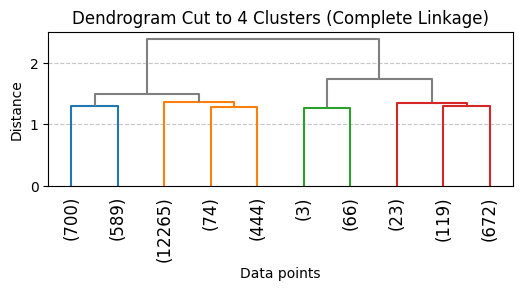
\includegraphics[width=\textwidth]{plots/dendrogram_complete.png}
        \caption{Complete Linkage Dendrogram}
        \label{fig:dendrogram_complete}
    \end{subfigure}
    \begin{subfigure}[b]{0.49\textwidth}
        \centering
        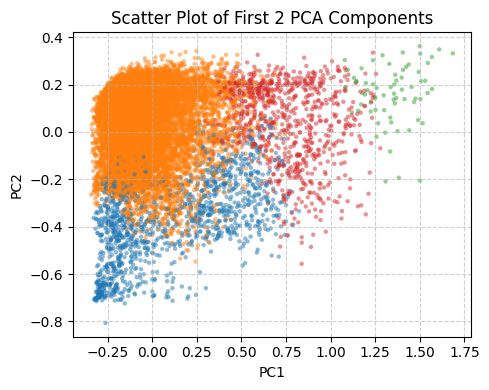
\includegraphics[width=\textwidth]{plots/scatter_complete.png}
        \caption{Complete Linkage Scatter plot}
        \label{fig:pairplot_ward_5}
    \end{subfigure}
    \caption{Dendrograms for hierarchical clustering with Complete Linkage}
    \label{fig:dendrograms_complete}
\end{figure}

\section{General considerations}\label{sec:considerations}
\textbf{PUNTI TRATTABILI (non in ordine):}

- k-means raggiunge valori alti di silhouette ma perchè le variabili usate sono poche - questo può essere
confrontato con ward's che usa invece più variabili (ma paragonabile per valore di silhouette? altrimenti fare confronto con metodo di hierarchical
che raggiunge performance simili a kmeans- anche se meno paragonabile rispetto a ward's perchè lui + simile a kmeans dato che usa sse)
--> vedere se dire in general considerations o se in k-means

- considerazioni generali su dataset, il clustering riesce a far emergere qualcosa riguardo alla struttura dei dati?

- k-means algoritmo più lineare mentre dbscan e hierarchical più complessi, che magari fanno emergere cose più interessanti

- confronto con titletype?

- se mettiamo hierarchical clustering come prima subsection, spiegare il perchè

- kmeans:
    - obiettivo → trovare cluster ben separati, con silhouette onesta e SSE bassa
    - risultato → 4 cluster ben separati, silhouette score di 0.315, SSE di 535.51
    - confrontabile con metodi di hierarchical?

- DBSCAN:
        OBIETTIVO → trovare miglior compromesso tra struttura interpretabile (almeno 2 cluster), poco rumore e silhouette onesta.  
        → e con cluster che anche se piccoli siano "effettivamente separati" 
        problema →per caratteristiche del dataset stesso → DBSCAN tende a formare un cluster dominante nella zona densa che "cattura" la maggior parte dei dati 
        (la classe maggioritaria) mentre dati + dispersi sono rappr come rumore o come micro-custer non significativi
        Spesso epsilon alta →  porta a un comportamento più "aggressivo" nell'unire punti, risultando nel "cluster gigante" 
        Tendenzialmente con epsilon più basso, l'algoritmo riesce a distinguere meglio le diverse densità,catturando sia la struttura principale che 
        eventuali sottogruppi significativi.
        "To conclude, these observations highlight DBSCAN's limitations when applied to datasets with skewed feature
        distributions and unbalanced local densities. Nonetheless, the exploration helped isolate parameter ranges where
        meaningful subclusters begin to emerge,beyond the dominant density mass."

